\documentclass{article}

\usepackage{graphicx}
\usepackage{tikz}
\usepackage{tikzsymbols}
\usetikzlibrary{calc,patterns,shapes.geometric}
\pagestyle{empty}
\usepackage[margin=0pt]{geometry}
\geometry{papersize={14in,12in}}

\def\centerarc[#1](#2)(#3:#4:#5){\draw[#1] ($(#2)+({#5*cos(#3)},{#5*sin(#3)})$) arc (#3:#4:#5);}

\begin{document}
	\begin{figure}
		\centering
		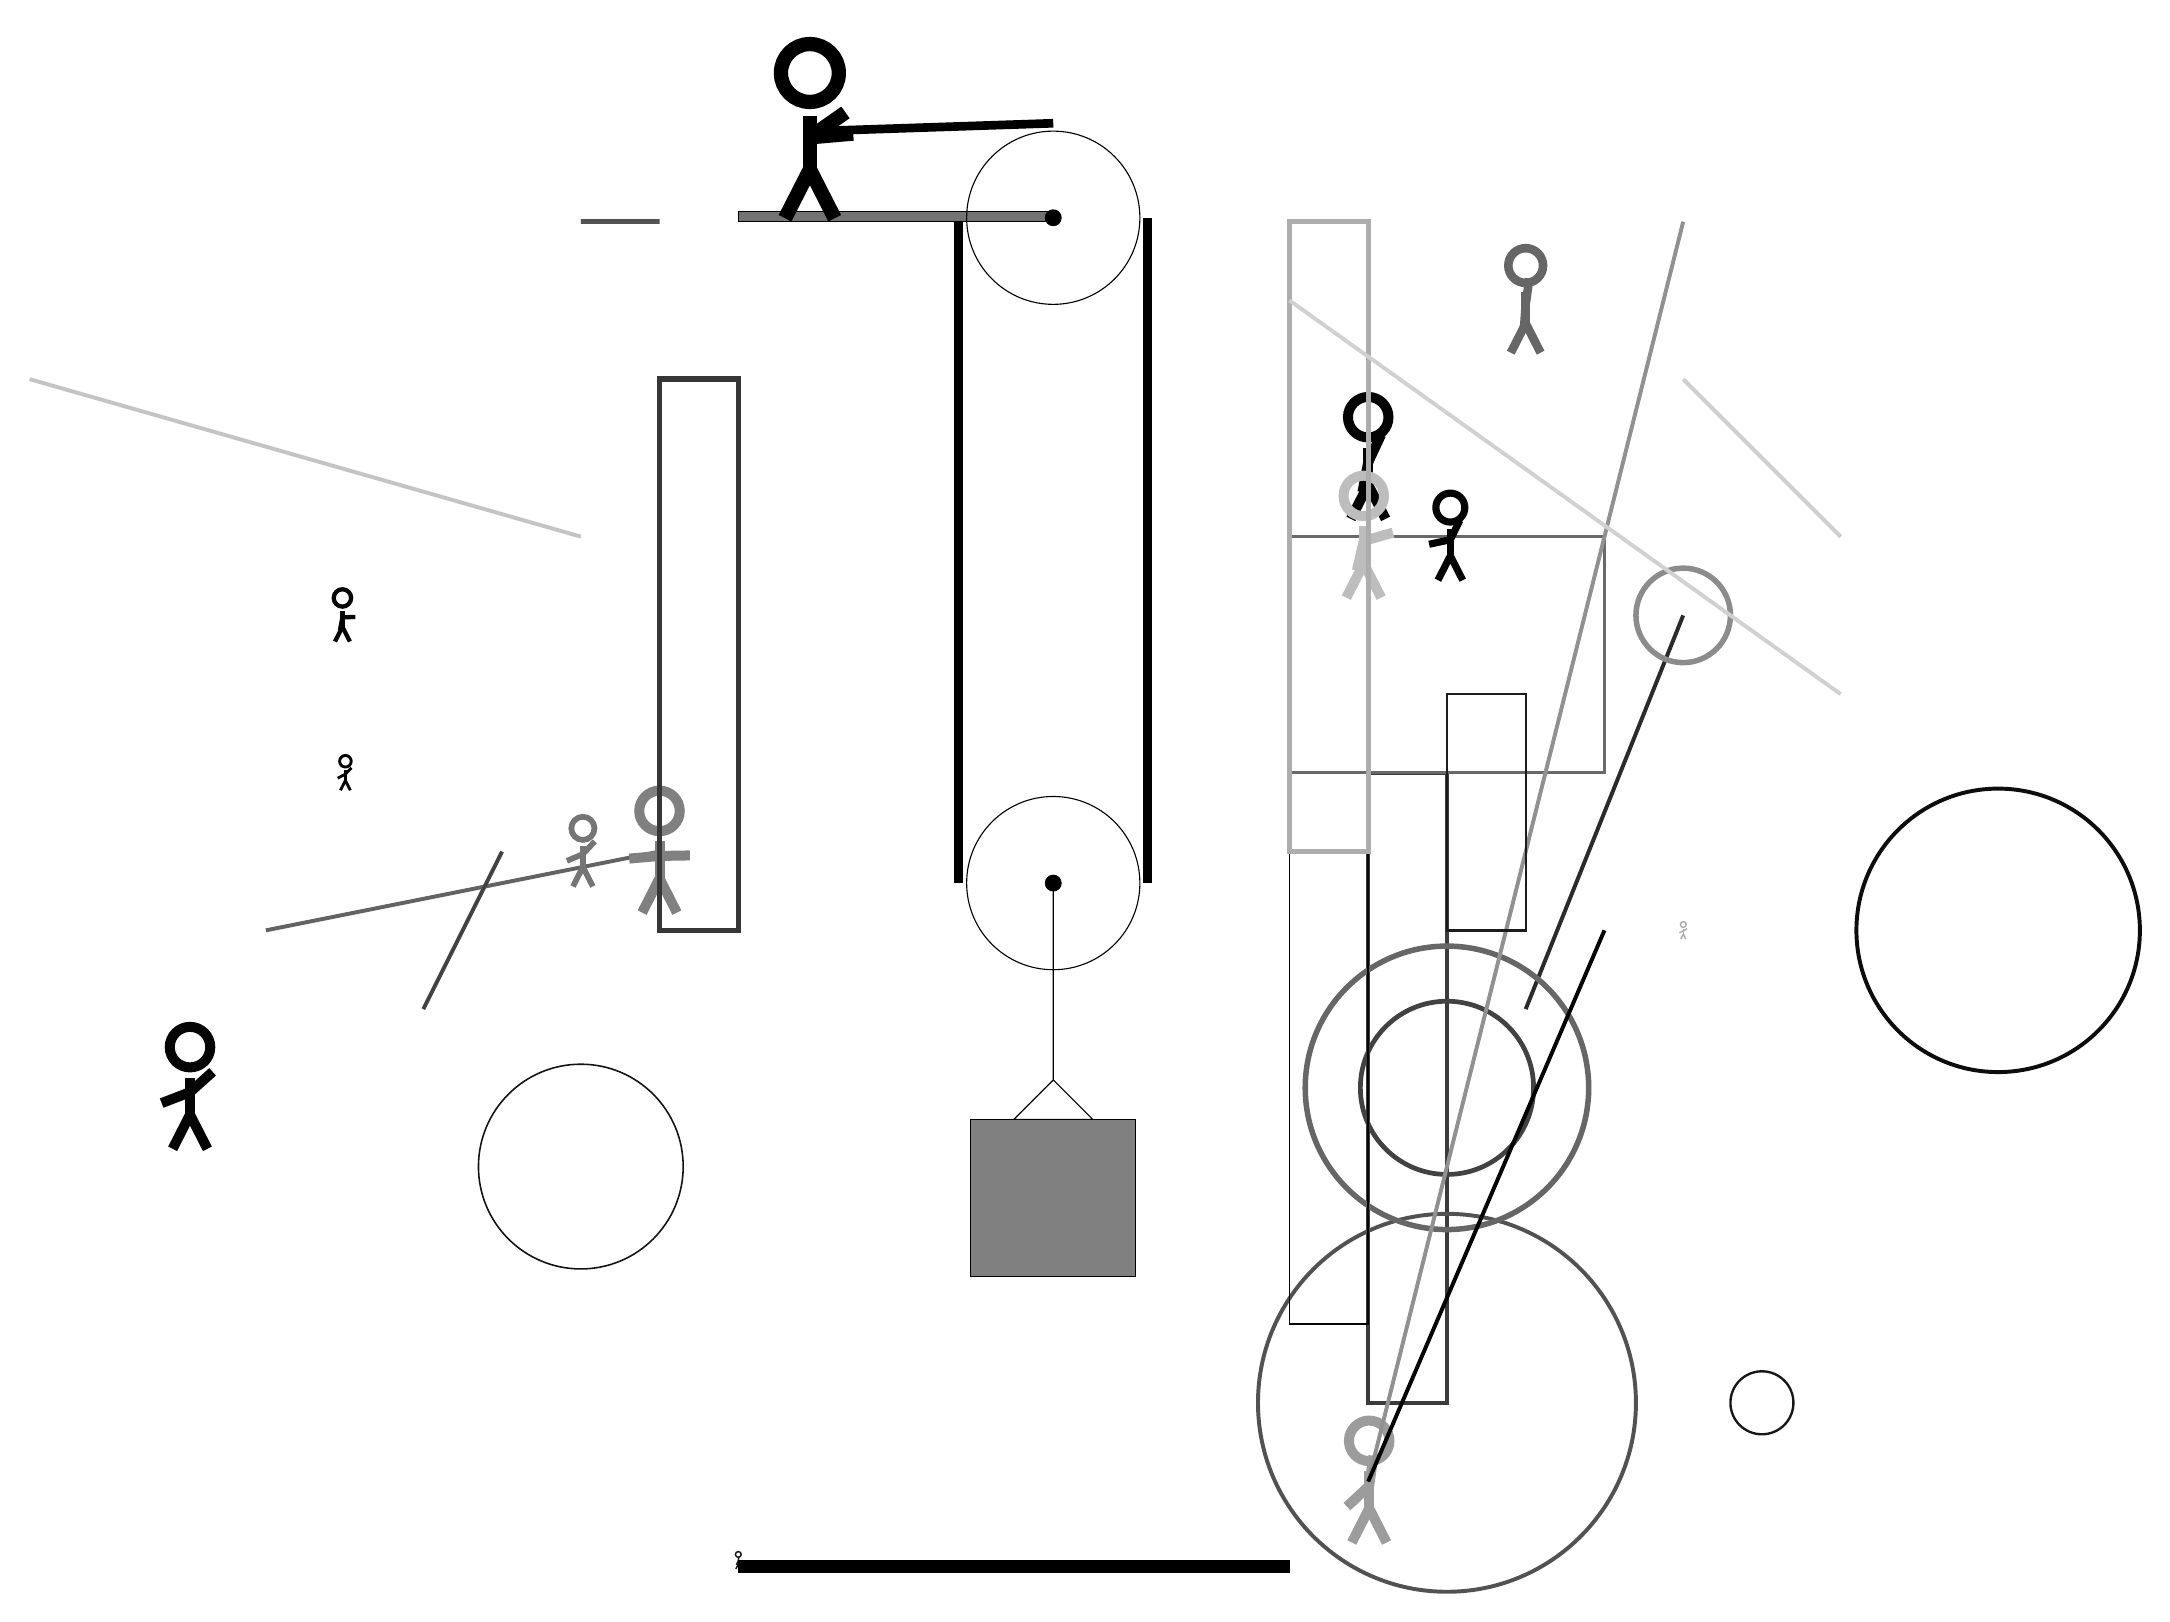
\begin{tikzpicture}
			%%%%% START %%%%%
			
			\draw[fill=black!55] (-2, 14) rectangle (2, 14.125);
			
			\draw (2, 5.6) circle (1.1);
			\draw[fill=black] (2, 5.6) circle (0.1);
			
			\draw (2, 14.05) circle (1.1);
			\draw[fill=black] (2, 14.05) circle (0.1);
			
			\draw (2, 5.6) -- (2, 3.1) -- (1.5, 2.6) -- (2.5, 2.6) -- (2, 3.1);
			\draw[fill=black!50] (0.95, 2.6) rectangle (3.05, 0.6);
			
			\draw[line width=1.1mm] (0.8, 14) -- (0.8, 5.6);
			\centerarc[line width=1.1mm](2, 5.6)(180:360:1.2000000000000002);
			\draw[line width=1.1mm](3.2, 5.6) -- (3.2, 14.05);
			\centerarc[line width=1.1mm](2, 14.05)(0:90:1.2000000000000002);
			\draw[line width=1.1mm](2, 15.25) -- (-1, 15.15);
			
			\node at (-1, 15.15) {\Strichmaxerl[10][-175][35]};
			
			\draw[line width=0.5mm, color=black!61](-3, 6) -- (-8, 5);
			
			\draw[line width=0.5mm, color=black!74](-6, 4) -- (-5, 6);
			\draw [line width=0.5mm, color=black!95](14, 5) circle (1.8);
			\node[line width=0.5mm, color=black!98] at (6, 11) {\Strichmaxerl[7][79][65]};
			
			\node[line width=0.3mm, color=black!92] at (-2, -3) {\Strichmaxerl[1][63][82]};
			\node[line width=0.7mm, color=black!39] at (6, -2) {\Strichmaxerl[7][43][82]};
			\draw [line width=0.3mm, color=black!91](11, -1) circle (0.4);
			
			\draw[line width=0.5mm, color=black!19](10, 12) -- (12, 10);
			\draw[line width=0.5mm, color=black!77] (6, -1) rectangle (7, 7);
			
			\draw[line width=0.5mm, color=black!83](10, 9) -- (8, 4);
			\draw[line width=0.4mm, color=black!59] (5, 7) rectangle (9, 10);
			\draw [line width=0.6mm, color=black!74](7, 3) circle (1.1);
			\draw [line width=0.7mm, color=black!45](10, 9) circle (0.6);
			
			\node[line width=0.4mm, color=black!99] at (7, 10) {\Strichmaxerl[5][12][64]};
			\node[line width=0.3mm, color=black!26] at (6, 10) {\Strichmaxerl[7][77][16]};
			\draw[line width=0.6mm, color=black!68] (-3, 14) rectangle (-4, 14);
			
			\draw [line width=0.5mm, color=black!68](7, -1) circle (2.4);
			\draw [line width=0.7mm, color=black!60](7, 3) circle (1.8);
			\node[line width=0.2mm, color=black!50] at (-3, 6) {\Strichmaxerl[7][5][1]};
			\draw[line width=0.5mm, color=black!43](6, -2) -- (10, 14);
			\draw[line width=0.3mm, color=black!89] (7, 5) rectangle (8, 8);
			
			\draw [line width=0.2mm, color=black!93](-4, 2) circle (1.3);
			\node[line width=0.6mm, color=black!98] at (-7, 9) {\Strichmaxerl[3][79][1]};
			\node[line width=0.3mm, color=black!98] at (-9, 3) {\Strichmaxerl[7][21][42]};
			\node[line width=0.5mm, color=black!100] at (-7, 7) {\Strichmaxerl[2][28][46]};
			
			\draw[line width=0.7mm, color=black!79] (-2, 5) rectangle (-3, 12);
			\draw[line width=0.2mm, color=black!98] (5, 0) rectangle (6, 14);
			\draw[line width=0.5mm, color=black!99](9, 5) -- (6, -2);
			\draw[line width=0.6mm, color=black!32] (5, 14) rectangle (6, 6);
			
			\node[line width=0.6mm, color=black!54] at (-4, 6) {\Strichmaxerl[4][23][47]};
			\node[line width=0.5mm, color=black!33] at (10, 5) {\Strichmaxerl[1][23][31]};
			\draw[line width=0.5mm, color=black!18](5, 13) -- (12, 8);
			\node[line width=0.2mm, color=black!60] at (8, 13) {\Strichmaxerl[6][86][82]};
			\draw[line width=0.5mm, color=black!23](-4, 10) -- (-11, 12);
			
			\draw[fill=black] (-2, -3) rectangle (5, -3.15);
			
			%%%%% END %%%%%
		\end{tikzpicture}
	\end{figure}	
\end{document}